\begin{figure}[!htb]
\centering
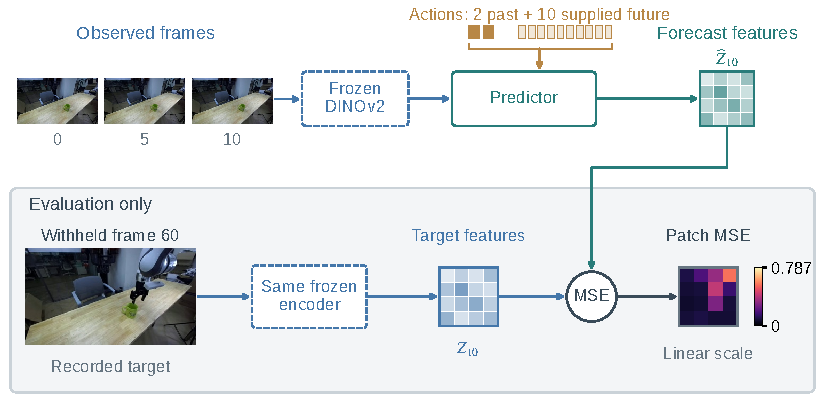
\includegraphics[width=\linewidth]{generated/editorial/task_refined.pdf}
\caption[Recorded inputs and evaluator-only target.]{\textbf{Available inputs and withheld evaluation targets.} Three observed frames (0, 5, 10), two past action blocks and ten supplied future blocks determine the feature forecast. Frame 60 enters only the evaluator through the same frozen DINOv2 encoder. One block spans five source-frame intervals, not seconds. Tiles are schematic feature grids; the heatmap is the actual three-seed standardized $h=10$ patch error for the prespecified median-by-episode-gain case's first window (MSE 0.1727; gain $-0.305\%$ versus autoregression). Its linear scale retains the original 0--0.787 range. Recorded DROID images are unchanged (CC BY 4.0); no RGB or robot actions are generated.}
\label{fig:spatial-task}
\end{figure}
